%=========================================================================
% Start of 
%=========================================================================
\preClass{Basic Trigonometry}

\begin{problem}
\item A circle of radius $r$ is centered at the origin, and a ray
  originates from the origin at a given angle, $\theta$. The ray
  passes through the circle at the coordinate $(x,y)$. A function of
  $\theta$ can be defined in terms of the coordinate.

  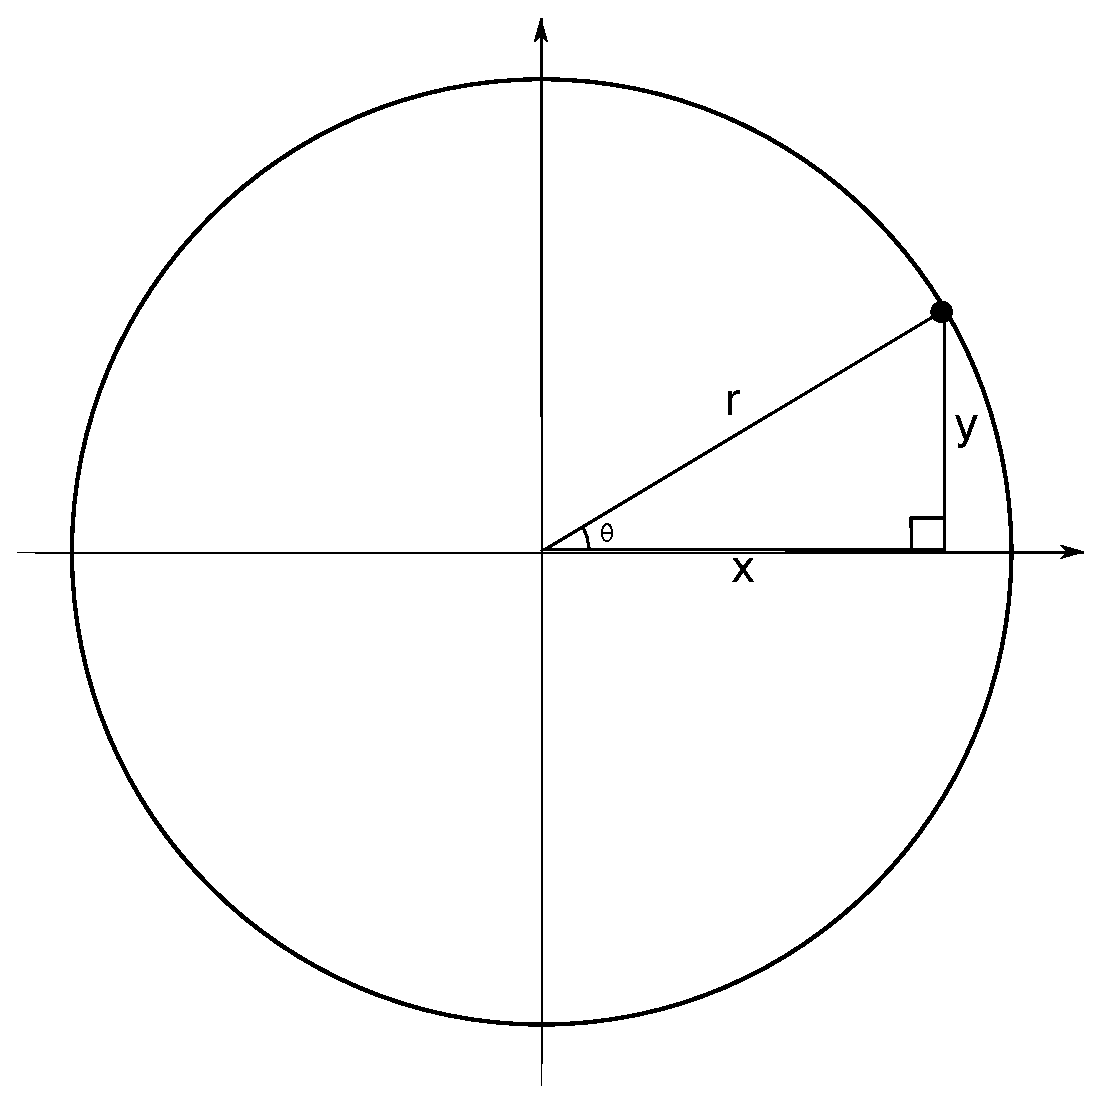
\includegraphics[width=8cm]{trig/img/circleTrig}

  \begin{subproblem}
  \item A function, sine, is defined to be
    \begin{eqnarray*}
      \sin(\theta) & = & \frac{y}{r}.
    \end{eqnarray*}
    Determine the formula for the value of $y$ given $r$ and $\theta$
    in terms of the sine function.
    \vfill
  \item A function, cosine, is defined to be
    \begin{eqnarray*}
      \cos(\theta) & = & \frac{x}{r}.
    \end{eqnarray*}
    Determine the formula for the value of $x$ given $r$ and $\theta$
    in terms of the cosine function.
    \vfill
  \end{subproblem}

\end{problem}


\actTitle{Basic Trigonomety}
\begin{problem}
\item Answer each of the following questions where the given point is $P(2,4)$.
  \begin{subproblem}
  \item Make a sketch of the coordinate plane and include the point
    $P(2,4)$. Draw the ray from the origin to the point. (Label your
    axes!)  \vfill
  \item Add a circle to your sketch show center is the origin and goes
    through the point. Label the angle $\theta$ as the angle between
    the ray and the $x$-axis.
  \item What is the radius of the circle?  
    \vspace{2em}
  \item Determine the values of the sine and cosine for the angle.
    \begin{eqnarray*}
      \sin(\theta) & = & \\ [10pt]
      \cos(\theta) & = & 
    \end{eqnarray*}
  \end{subproblem}

\clearpage

\item For each point below determine the radius and the value of the
  sine and cosine of the angle associated with each point.
  \begin{subproblem}
  \item $P(1,0)$
    \vfill
  \item $P(0,1)$
    \vfill
  \item $P(-1,0)$
    \vfill
  \item $P(0,-1)$
    \vfill
  \item $P\left(\frac{\sqrt{2}}{2},\frac{\sqrt{2}}{2}\right)$
    \vfill
  \end{subproblem}

\clearpage

\item The circle below is centered at the origin and has a radius of
  one.

  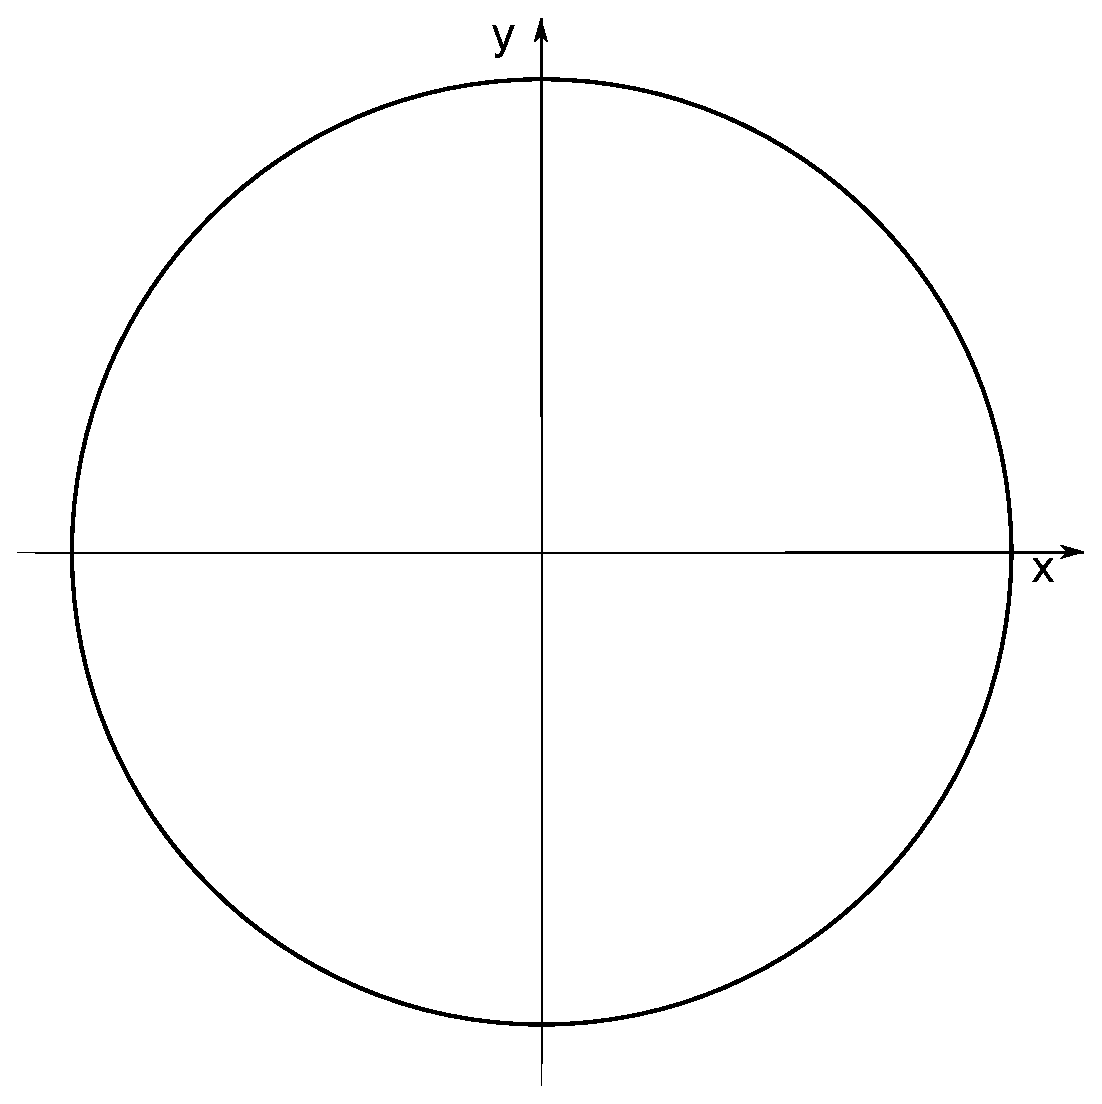
\includegraphics[width=16cm]{trig/img/blankCircle}

  \begin{subproblem}
  \item Mark the locations on the circle whose associated angles are
    0, $\pi/4$, $\pi/2$, $3\pi/4$, $\pi$, $5\pi/4$, $3\pi/2$, and
    $7\pi/4$.
    \clearpage

  \item Determine the $(x,y)$ coordinates for each angle.
    \vfill
  \item Determine the cosine and sine of each angle.
    \vfill
  \end{subproblem}

\end{problem}

\postClass

\begin{problem}
\item Briefly state two ideas from today's class.
  \begin{itemize}
  \item 
  \item 
  \end{itemize}
\item 
  \begin{subproblem}
    \item
  \end{subproblem}
\end{problem}


\propertiesTitle{The Unit Circle}

\begin{minipage}{0.5\linewidth}
  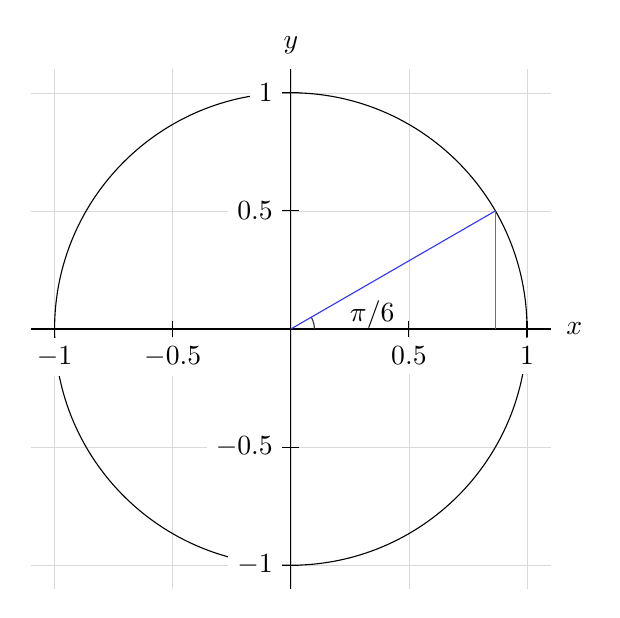
\begin{tikzpicture}[scale=3]
    \draw[step=0.5cm,gray!30,very thin] (-1.1,-1.1) grid (1.1,1.1);
    \draw (-1.1,0) -- (1.1,0); \draw (0,-1.1) -- (0,1.1); 
    \draw (0,0) circle [radius=1cm];

    \draw[black!80,thin] (.1cm,0cm) arc [start angle=0, end angle=30,radius=.1cm]; 
    \draw[red!80,thin] (30:1cm) -- ++(0,-0.5cm); 
    \draw[blue!80,thin] (0,0) -- (30:1cm); 
    \draw (10:0.35cm) node {$\pi/6$};
    \draw (0,1.2cm) node {$y$};
    \draw (1.2cm,0) node {$x$};

    \foreach \x in {-1,-0.5,0.5,1} 
       \draw (\x cm,1pt) -- (\x cm,-1pt) node[anchor=north,fill=white] {$\x$}; 
    \foreach \y in {-1,-0.5,0.5,1} 
       \draw (1pt,\y cm) -- (-1pt,\y cm) node[anchor=east,fill=white] {$\y$};
  \end{tikzpicture}
\end{minipage}
\begin{minipage}{0.5\linewidth}
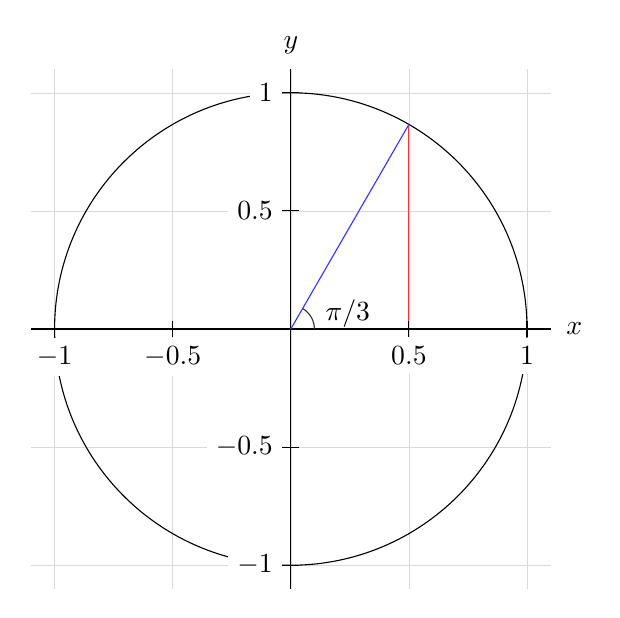
\begin{tikzpicture}[scale=3]
\draw[step=0.5cm,gray!30,very thin] (-1.1,-1.1) grid (1.1,1.1);
\draw (-1.1,0) -- (1.1,0);
\draw (0,-1.1) -- (0,1.1);
\draw (0,0) circle [radius=1cm];

\draw[black!80,thin] (.1cm,0cm) arc [start angle=0, end angle=60,radius=.1cm];
\draw[red!80,thin] (0.5,0) -- (60:1cm);
\draw[blue!80,thin] (0,0) -- (60:1cm);
\draw (15:0.25cm) node {$\pi/3$};
\draw (0,1.2cm) node {$y$};
\draw (1.2cm,0) node {$x$};

\foreach \x in {-1,-0.5,0.5,1}
   \draw (\x cm,1pt) -- (\x cm,-1pt) node[anchor=north,fill=white] {$\x$};
\foreach \y in {-1,-0.5,0.5,1}
   \draw (1pt,\y cm) -- (-1pt,\y cm) node[anchor=east,fill=white] {$\y$};
\end{tikzpicture}
\end{minipage}

\begin{minipage}{0.5\linewidth}
  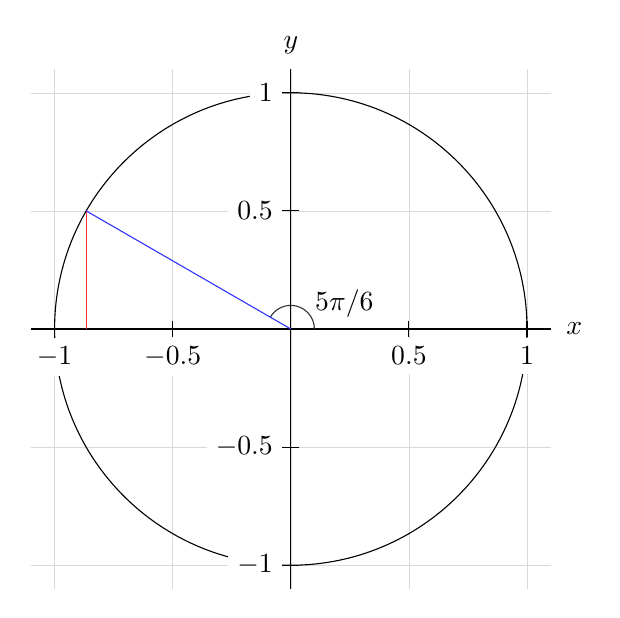
\begin{tikzpicture}[scale=3]
    \draw[step=0.5cm,gray!30,very thin] (-1.1,-1.1) grid (1.1,1.1);
    \draw (-1.1,0) -- (1.1,0); 
    \draw (0,-1.1) -- (0,1.1); \draw (0,0) circle [radius=1cm];

    \draw[black!80,thin] (.1cm,0cm) arc [start angle=0, end angle=150,radius=.1cm]; 
    \draw[red!80,thin] (150:1cm) -- ++(0,-0.5cm); 
    \draw[blue!80,thin] (0,0) -- (150:1cm); 
    \draw (25:0.25cm) node {$5\pi/6$};
    \draw (0,1.2cm) node {$y$};
    \draw (1.2cm,0) node {$x$};

    \foreach \x in {-1,-0.5,0.5,1} 
       \draw (\x cm,1pt) -- (\x cm,-1pt) node[anchor=north,fill=white] {$\x$}; 
    \foreach \y in {-1,-0.5,0.5,1} 
    \draw (1pt,\y cm) -- (-1pt,\y cm) node[anchor=east,fill=white] {$\y$};
  \end{tikzpicture}
\end{minipage}
\begin{minipage}{0.5\linewidth}
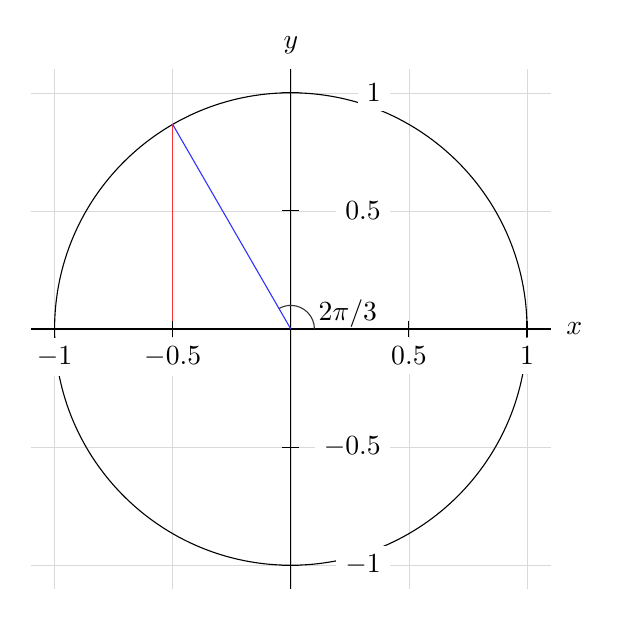
\begin{tikzpicture}[scale=3]
\draw[step=0.5cm,gray!30,very thin] (-1.1,-1.1) grid (1.1,1.1);
\draw (-1.1,0) -- (1.1,0);
\draw (0,-1.1) -- (0,1.1);
\draw (0,0) circle [radius=1cm];

\draw[black!80,thin] (.1cm,0cm) arc [start angle=0, end angle=120,radius=.1cm];
\draw[red!80,thin] (-0.5,0) -- (120:1cm);
\draw[blue!80,thin] (0,0) -- (120:1cm);
\draw (15:0.25cm) node {$2\pi/3$};
\draw (0,1.2cm) node {$y$};
\draw (1.2cm,0) node {$x$};

\foreach \x in {-1,-0.5,0.5,1}
   \draw (\x cm,1pt) -- (\x cm,-1pt) node[anchor=north,fill=white] {$\x$};
\foreach \y in {-1,-0.5,0.5,1}{
   \draw (-1pt,\y cm) -- (1pt,\y cm);
   \draw (12pt,\y cm) node[anchor=east,fill=white] {$\y$};
 }
\end{tikzpicture}
\end{minipage}

\clearpage

\begin{minipage}{0.5\linewidth}
  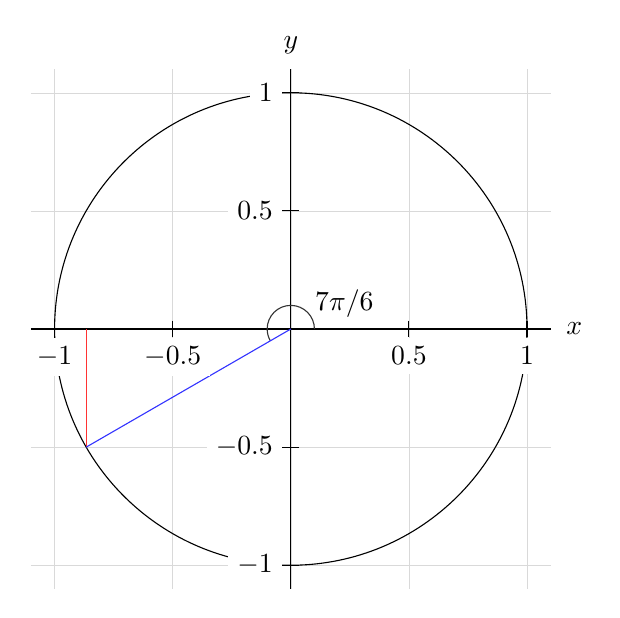
\begin{tikzpicture}[scale=3]
    \draw[step=0.5cm,gray!30,very thin] (-1.1,-1.1) grid (1.1,1.1);
    \draw (-1.1,0) -- (1.1,0); 
    \draw (0,-1.1) -- (0,1.1); \draw (0,0) circle [radius=1cm];

    \draw[black!80,thin] (.1cm,0cm) arc [start angle=0, end angle=210,radius=.1cm]; 
    \draw[red!80,thin] (210:1cm) -- ++(0,0.5cm); 
    \draw[blue!80,thin] (0,0) -- (210:1cm); 
    \draw (25:0.25cm) node {$7\pi/6$};
    \draw (0,1.2cm) node {$y$};
    \draw (1.2cm,0) node {$x$};

    \foreach \x in {-1,-0.5,0.5,1} 
       \draw (\x cm,1pt) -- (\x cm,-1pt) node[anchor=north,fill=white] {$\x$}; 
    \foreach \y in {-1,-0.5,0.5,1} 
    \draw (1pt,\y cm) -- (-1pt,\y cm) node[anchor=east,fill=white] {$\y$};
  \end{tikzpicture}
\end{minipage}
\begin{minipage}{0.5\linewidth}
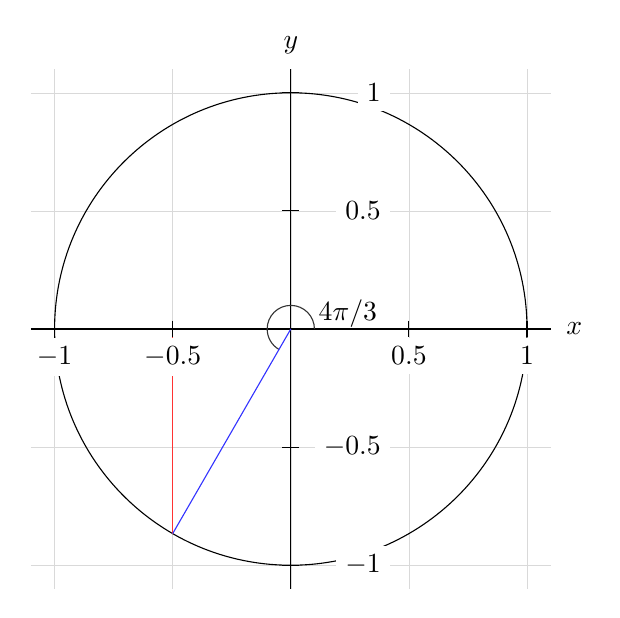
\begin{tikzpicture}[scale=3]
\draw[step=0.5cm,gray!30,very thin] (-1.1,-1.1) grid (1.1,1.1);
\draw (-1.1,0) -- (1.1,0);
\draw (0,-1.1) -- (0,1.1);
\draw (0,0) circle [radius=1cm];

\draw[black!80,thin] (.1cm,0cm) arc [start angle=0, end angle=240,radius=.1cm];
\draw[red!80,thin] (-0.5,0) -- (240:1cm);
\draw[blue!80,thin] (0,0) -- (240:1cm);
\draw (15:0.25cm) node {$4\pi/3$};
\draw (0,1.2cm) node {$y$};
\draw (1.2cm,0) node {$x$};

\foreach \x in {-1,-0.5,0.5,1}
   \draw (\x cm,1pt) -- (\x cm,-1pt) node[anchor=north,fill=white] {$\x$};
\foreach \y in {-1,-0.5,0.5,1}{
   \draw (-1pt,\y cm) -- (1pt,\y cm);
   \draw (12pt,\y cm) node[anchor=east,fill=white] {$\y$};
 }
\end{tikzpicture}
\end{minipage}


\begin{minipage}{0.5\linewidth}
  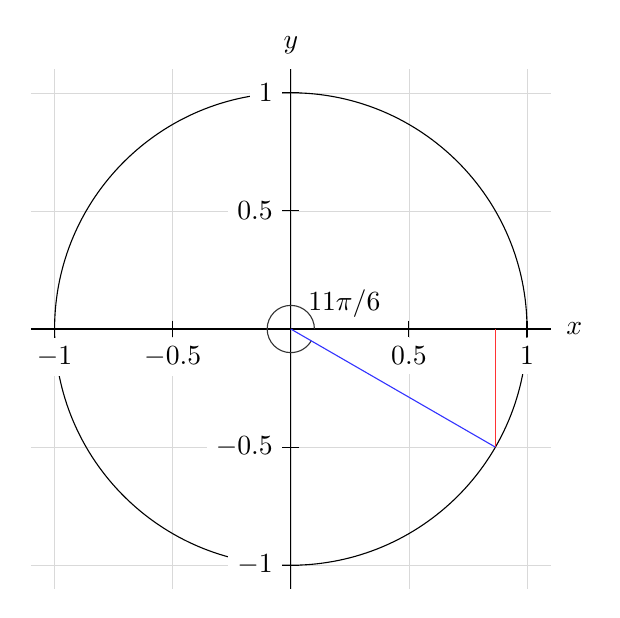
\begin{tikzpicture}[scale=3]
    \draw[step=0.5cm,gray!30,very thin] (-1.1,-1.1) grid (1.1,1.1);
    \draw (-1.1,0) -- (1.1,0); 
    \draw (0,-1.1) -- (0,1.1); \draw (0,0) circle [radius=1cm];

    \draw[black!80,thin] (.1cm,0cm) arc [start angle=0, end angle=330,radius=.1cm]; 
    \draw[red!80,thin] (330:1cm) -- ++(0,0.5cm); 
    \draw[blue!80,thin] (0,0) -- (330:1cm); 
    \draw (25:0.25cm) node {$11\pi/6$};
    \draw (0,1.2cm) node {$y$};
    \draw (1.2cm,0) node {$x$};

    \foreach \x in {-1,-0.5,0.5,1} 
       \draw (\x cm,1pt) -- (\x cm,-1pt) node[anchor=north,fill=white] {$\x$}; 
    \foreach \y in {-1,-0.5,0.5,1} 
    \draw (1pt,\y cm) -- (-1pt,\y cm) node[anchor=east,fill=white] {$\y$};
  \end{tikzpicture}
\end{minipage}
\begin{minipage}{0.5\linewidth}
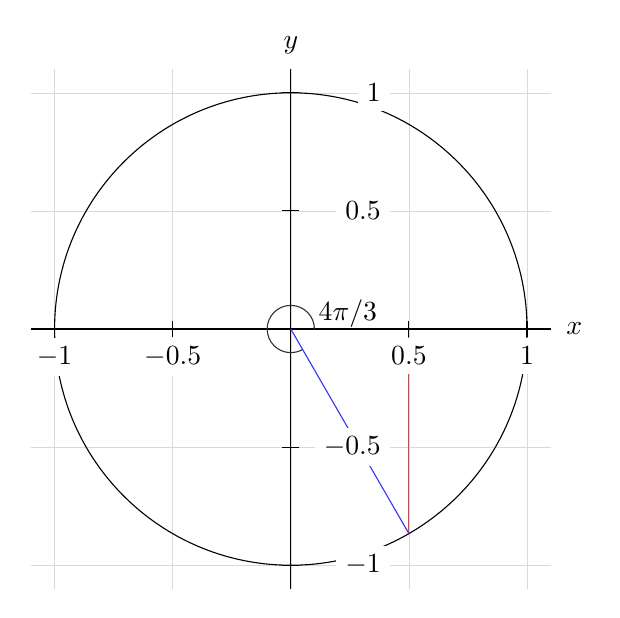
\begin{tikzpicture}[scale=3]
  \draw[step=0.5cm,gray!30,very thin] (-1.1,-1.1) grid (1.1,1.1);
  \draw (-1.1,0) -- (1.1,0);
  \draw (0,-1.1) -- (0,1.1);
  \draw (0,0) circle [radius=1cm];

  \draw[black!80,thin] (.1cm,0cm) arc [start angle=0, end angle=300,radius=.1cm];
  \draw[red!80,thin] (0.5,0) -- (300:1cm);
  \draw[blue!80,thin] (0,0) -- (300:1cm);
  \draw (15:0.25cm) node {$4\pi/3$};
  \draw (0,1.2cm) node {$y$};
  \draw (1.2cm,0) node {$x$};

  \foreach \x in {-1,-0.5,0.5,1}
    \draw (\x cm,1pt) -- (\x cm,-1pt) node[anchor=north,fill=white] {$\x$};
  \foreach \y in {-1,-0.5,0.5,1}{
      \draw (-1pt,\y cm) -- (1pt,\y cm);
      \draw (12pt,\y cm) node[anchor=east,fill=white] {$\y$};
  }
\end{tikzpicture}
\end{minipage}


%%% Local Variables:
%%% mode: latex
%%% TeX-master: "../labManual"
%%% End:

